\documentclass[serif,mathserif]{beamer}
\usepackage{amsmath, amsfonts, epsfig, xspace}
\usepackage{algorithm,algorithmic}
\usepackage{pstricks,pst-node}
\usepackage{multimedia}
\usepackage[normal,tight,center]{subfigure}
\setlength{\subfigcapskip}{-.5em}
\usepackage{beamerthemesplit}
\usetheme{lankton-keynote}

\author[0d1n web hacking tool]{ Tool designed for bruteforcing Web Applications \quad 
\includegraphics[width=3cm]{images/odin.png} }

\title[ Page \hspace{2em}\insertframenumber/\inserttotalframenumber]{0d1n Web Hacking tool}

\date{February 8, 2015} 

\institute{Antonio Costa - CoolerVoid - c00f3r[aT]gmail[DOt]com}

\begin{document}

\maketitle

% \section{Introduction}  % add these to see outline in slides



\begin{frame}
  \frametitle{Whoami}
  Author:
  \begin{itemize}  \item  Antonio Costa "CoolerVoid" is a Computer Programmer who loves the Hacker culture, he work as a system analyst at CONVISO for three years. Antonio working with code review, pentest and security research with focused on Secure Web Applications and Reverse Engineering.  He also has been speaking at in some Brazilian Security Conferences such as YSTS, OWASP Florianopolis and Bsides Sao Paulo.
  \end{itemize}
  \begin{figure}[t]
    \centering
    \subfigure[]{
%    \includegraphics[width=3cm]{figures/naked_leaves/00000240}}
    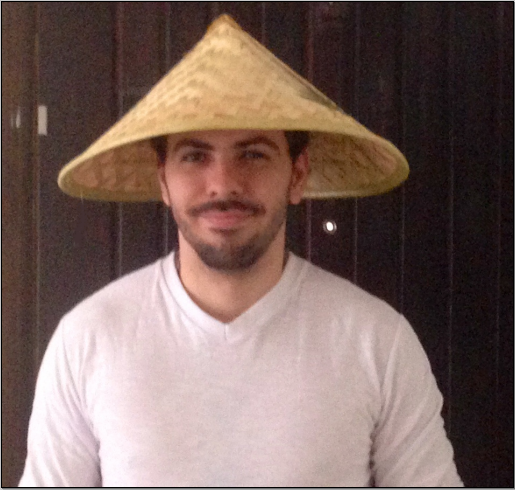
\includegraphics[width=4cm]{images/tony.png}}
  \end{figure}
\end{frame}


\begin{frame}
  \frametitle{Introduction}
  Software Information:
  \begin{itemize}
  \item  0d1n is a Open Source web application bruteforcer and Fuzzer,  it’s objective is to automate exhaustive tests to search anomalies. At other point view this anomalies can be a vulnerability, These tests can  follow web parameters, files, directories, forms and others. 
  \item  0d1n held by GPL v3 license: https://github.com/CoolerVoid/0d1n/blob/master/LICENSE.txt
  \end{itemize}
\end{frame}



\begin{frame}
  \frametitle{Introduction}
  Why is this tool made in C language ?
  \begin{itemize}
  \item  C has a high delay time for writing and debugging, but no pain no gain, it has a fast performance, in addition, the C language is run at any architecture like Mips,ARM and others... in the future can follow mobile implementations. Other benefits of C  is that it has good and high profile to write optimizations, if you want to write some lines in ASSEMBLY code with AES-NI or SiMD instructions, this is a good choice. 
  \item  Why you don't use POO ? in this project i follow "KISS" principe: http://pt.wikipedia.org/wiki/Keep\_It\_Simple
  \item  C language has a lot of old school dudes like a kernel hackers... 
  \end{itemize}
\end{frame}



\begin{frame}
  \frametitle{Introduction}
  Requirements:
  \begin{itemize}
  \item  Need "GCC" and "make" 
  \item  You must install "libcurl" 
  \item  Search libcurl-devel or libcurl-dev in your portage
  \item  Current version tested only Unix Like systems(Linux, MacOS and *BSD).
  \item  Current version run well, but is a BeTa version, you can report bug here: https://github.com/CoolerVoid/0d1n/issues 
  \end{itemize}
\end{frame}

% \section{Main Body} % add these to see outline in slides

\begin{frame}
  \frametitle{How you can use it}
  Following this to get, decompress, compile and execute:
  \begin{itemize}
  \item wget https://github.com/CoolerVoid/0d1n/archive/master.zip; 
  \item unzip master.zip; cd 0d1n-master; make; ./0d1n
  \end{itemize}
\end{frame}

\begin{frame}
  \frametitle{First overview at parameters}
  \begin{figure}[t]
    \centering
    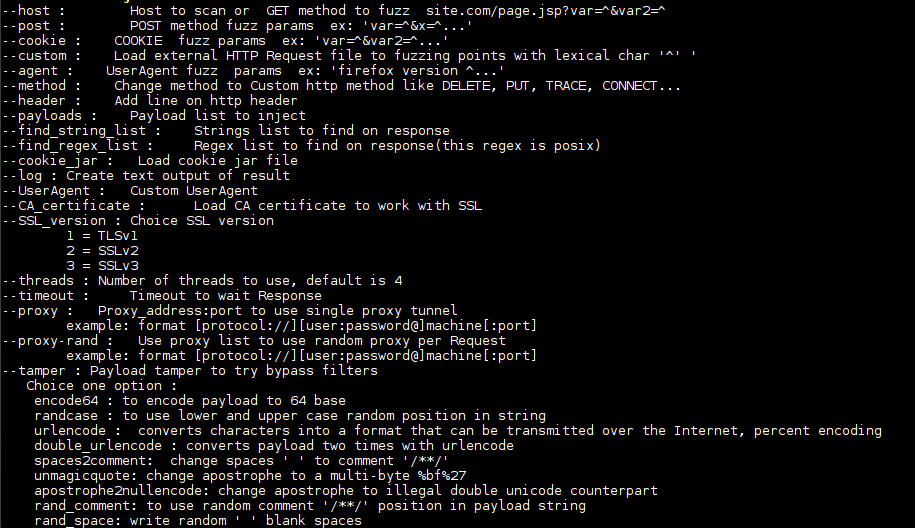
\includegraphics[width=12cm]{images/overview1.png}
  \end{figure}
\end{frame}

\begin{frame}
  \frametitle{First overview at parameters}
  Rules you need know about parameters:
  \begin{itemize}
  \item Each parameter is a resource function to help you
  \item When you view caracter  ' \^\ '(circumflex)  this is lexical caracter this represent the payload to replace each line in text file 
  \item The parameter "--log" you need use always 
  \item The parameter "--host" you need use always
  \item The parameter "--save\_response" if you use on end command, save Responses of requests, so if you click in "status code" at javascript table you can view response with highlights  
  \end{itemize}
\end{frame}

\begin{frame}
  \frametitle{First overview at parameters}
  Tamper resource:
  \begin{itemize}
  \item Tamper is a function to use camouflage in your payload, this way you can try bypass web application firewall
  \item Each options use different technique to try hide payload 
  \item You need to remember to using proxy list per Request to try walk in stealth to work without blacklists.  
  \begin{figure}[t]
    \centering
    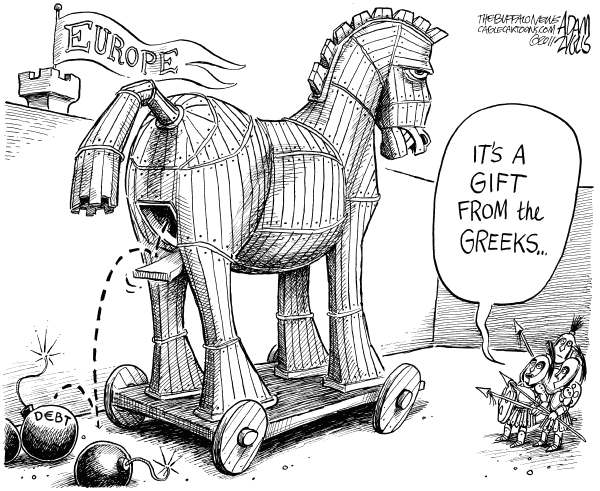
\includegraphics[width=7cm]{images/gift2.jpg}
  \end{figure}
 \end{itemize}
\end{frame}


\begin{frame}
  \frametitle{Example on XSS Attack}
  At test.php file you can view this source code, look don't have sanitization at POST input:
  \begin{itemize}
  \begin{figure}[t]
    \centering
    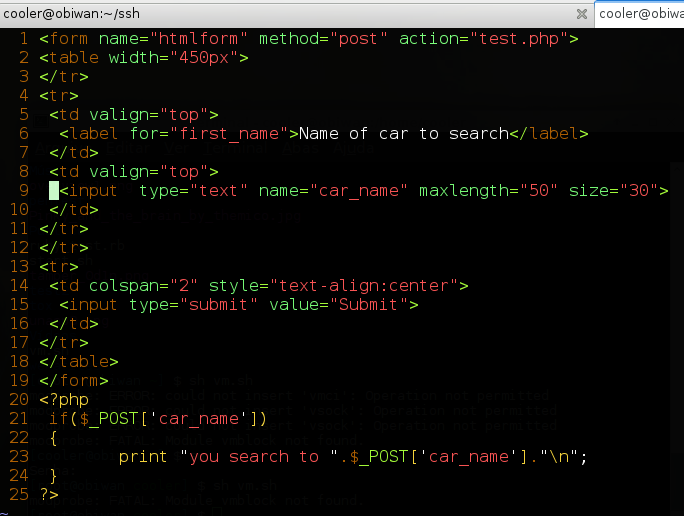
\includegraphics[width=9cm]{images/code_test_php.png}
  \end{figure}
 \end{itemize}
\end{frame}


\begin{frame}
  \frametitle{Example on XSS Attack}
  If you upload at your HTTP server, when rendering with browser return this following:
  \begin{itemize}
  \begin{figure}[t]
    \centering
    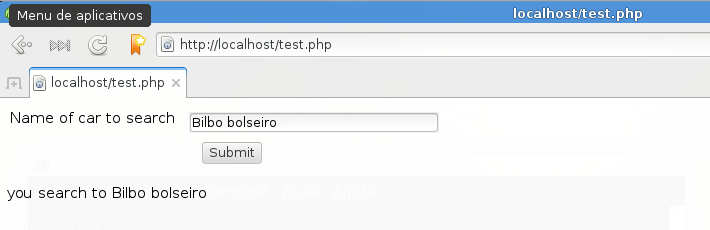
\includegraphics[width=10cm]{images/test_php.png}
  \end{figure}
 \end{itemize}
\end{frame}


\begin{frame}
  \frametitle{Example on XSS Attack}
  Following this to test application:
  \begin{itemize}
  \item ./0d1n --host http://localhost/test.php --post "car\_name=\^ \ " --payloads payloads/xss.txt --find\_regex\_list payloads/guess.txt --log name\_log --save\_response 
 \end{itemize}
\end{frame}



\begin{frame}
  \frametitle{Example on XSS Attack}
  Result of command generate HTML file with javascript table:
  \begin{itemize}
  \begin{figure}[t]    
    \centering
    \subfigure[First Frame]{
    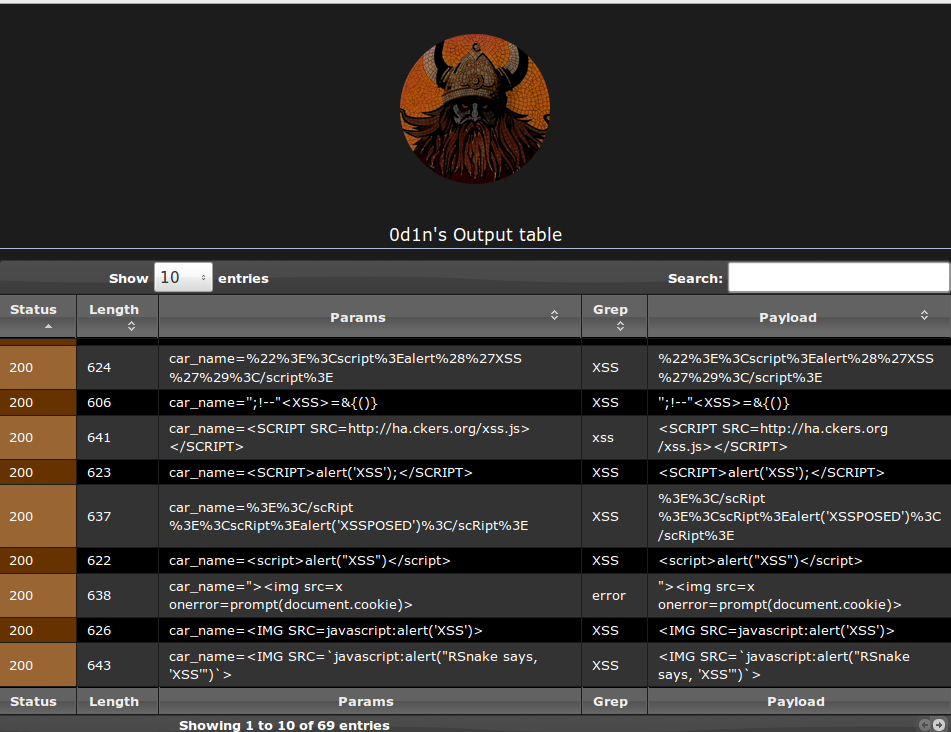
\includegraphics[width=10cm]{images/tables.png} }
  \end{figure}
 \end{itemize}
\end{frame}



\begin{frame}
  \frametitle{Example on XSS Attack}
  If you click at the number of Status you can view response with highlights:
  \begin{itemize}
  \begin{figure}[t]    
    \centering
    \subfigure[First Frame]{
    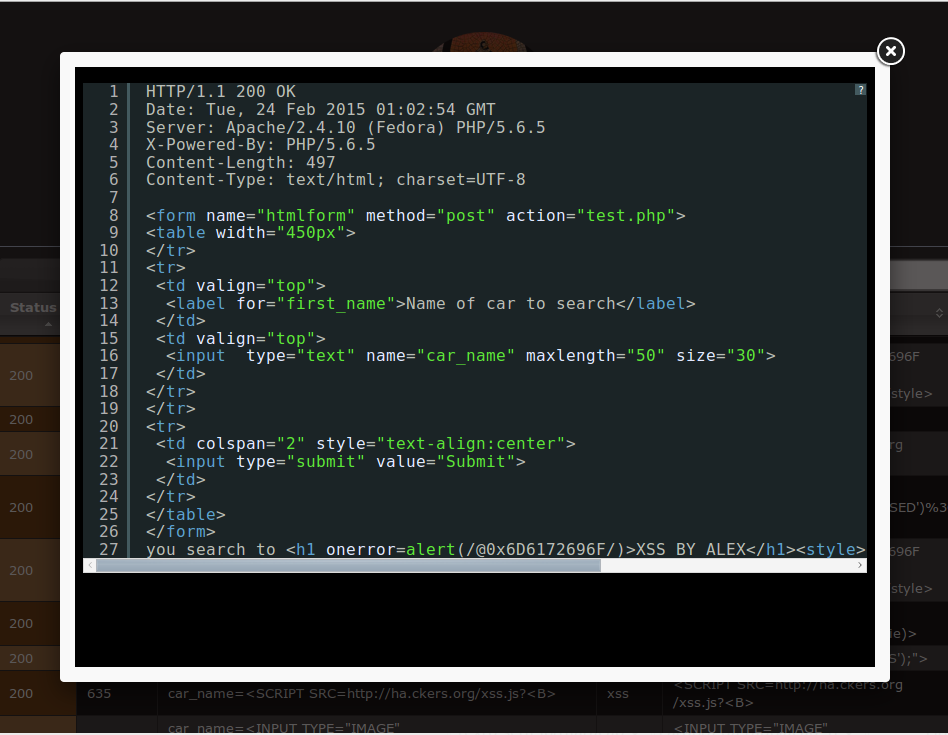
\includegraphics[width=10cm]{images/codehighlight.png} }
  \end{figure}
 \end{itemize}
\end{frame}



\begin{frame}
  \frametitle{Example on XSS Attack}
  Other way to test, you can use your custom request on external file:
  \begin{itemize}
  \begin{figure}[]    
    \centering
    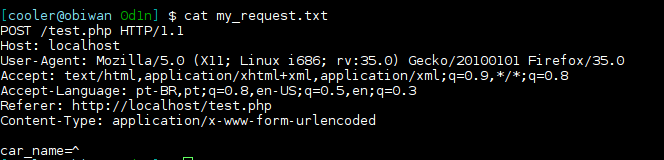
\includegraphics[width=10cm]{images/custom.png} 
  \end{figure}
 \end{itemize}
\end{frame}



\begin{frame}
  \frametitle{Example on XSS Attack}
  You can follow this command to make custom fuzzing:
  \begin{itemize}
   \item  ./0d1n --host http://localhost/ --custom my\_request.txt --payloads payloads/xss.txt --find\_regex\_list payloads/guess.txt  --log 133oooo5 --save\_response --timeout 5
  \end{itemize}
\end{frame}




\begin{frame}
  \frametitle{Frenetic questions}
  \begin{itemize}
  \item How do i enter in auth to fuzz other application ? You need Load cookie jar file.
  \item how do i use multiples special chars \^ \ to fuzz more parameters ? Yes you can do it, put more chars \^ \ in the parameters.
  \item how many threads can i use ? Depend of your machine, i recommend don't send a lot of requests for the server, because this is a deep pitfall you can get down the server, if server runs in production you may lost money and this is not good...
  \item  Do you have any doubts ? e-mail me...
  \end{itemize}
\end{frame}

\begin{frame}
  \frametitle{The End}
  \begin{figure}[]    
    \centering
    
\includegraphics[width=6cm]{images/letsgoplanet.jpg} 
  \end{figure}
\end{frame}



% \section{Conclusion} % add these to see outline in slides

\begin{frame}
  \frametitle{Greets}
  \begin{itemize}
  \item IAK, Sigsegv, M0nad, Slyfunky , RaphaelSC, pl4nkton, gustavoRobertux, Muzgo, Mente binaria, Otacon...
  \item HB, F-117, Eremita, Clandestine, Loganbr, Geyslan, Clodonil Trigo...
  \item my parents and friends...
  \item https://conviso.com.br/index.php/EN
  \end{itemize}
\end{frame}

\begin{frame}
  \frametitle{at construction...}
\end{frame}

\end{document}
